\section{Single-tank Water Tank}
\label{sec:singletank}

\subsection{Example Description}
\label{sec:singletank_desc}

The single-tank water tank pilot study is a simple example that comprises a single water tank which is controlled by a cyber controller. When the water level of the tank reaches a particular level (defined in the controller) the controller sends a command to the tank to empty using an exit valve. A diagram of the example is shown in Figure~\ref{fig:singletankoverview}. 
This pilot is also related to the next pilot in Section~\ref{sec:threetank}. 

\begin{figure}[htbp]
\begin{center}
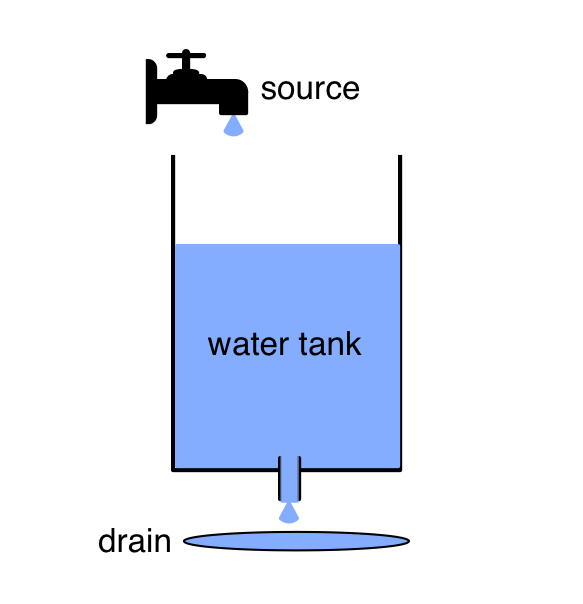
\includegraphics[width=0.4\textwidth]{singletank/singletank}
\caption{Overview of the single-tank water tank example}
\label{fig:singletankoverview}
\end{center}
\end{figure}

\subsection{Usage}
\label{sec:singletank_usage}

The example is available from the INTO-CPS application menu at \emph{File>Import Example Project} or at \url{https://github.com/INTO-CPS-Association/example-single_watertank} in the \emph{master} branch. There are several subfolders for the various elements: \texttt{FMU} contains the various FMUs of the study; \texttt{Models} -- contains the constituent models defined using the INTO-CPS simulation technologies; \texttt{Multi-models} -- contains the multi-model definition;  and \texttt{SysML} -- contains the SysML model defined for the study.

The \texttt{case-study\_single\_watertank} folder can be opened in the INTO-CPS application to run the various co-simulations as detailed in this document. To run a simulation, expand one of the multi-models and click `Simulate' for an experiment. 

%\subsection{INTO-CPS Technology}
%\label{sec:singletank_into}
%
%
%We demonstrate the use of the INTO-CPS SysML profile in Section~\ref{sec:singletank_into_sys}. Based upon the design architecture defined using the SysML profile, a multi-model is constructed in Section~\ref{sec:singletank_into_mm} along with the defined connections. The study is also used to demonstrate the Co-Simulation Orchestration Engine (COE) in Section~\ref{sec:singletank_into_co}. 

\subsection{INTO-CPS SysML profile}
\label{sec:singletank_into_sys}

The single tank SysML model produced using the INTO-CPS profile comprises two diagrams; an Architecture Structure Diagram (ASD) and a Connections Diagram (CD). 

The ASD in Figure~\ref{fig:fig:singletankasd} shows the system composition in terms of component subsystems from the perspective of multi-modelling. 

\begin{figure}[htbp]
\begin{center}
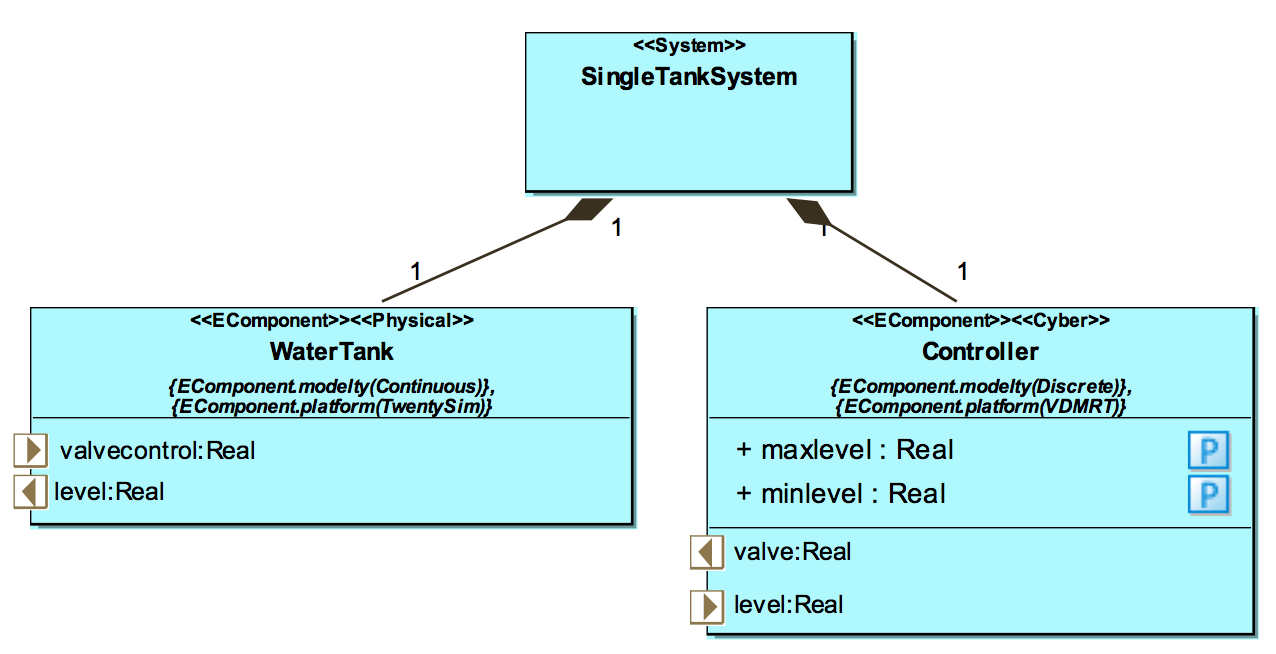
\includegraphics[width=0.8\textwidth]{singletank/sysml_asd.png}
\caption{Architecture Structure Diagram defining the Single-tank Water Tank system composition}
\label{fig:fig:singletankasd}
\end{center}
\end{figure}

This \emph{SingleTankSystem} model, comprises  a single \emph{WaterTank} physical component and  a cyber component \emph{Controller}. Ports are exposed by the  \emph{WaterTank} component for outputting the current water level (\texttt{level}) and for receiving valve control commands (\texttt{valvecontrol}). The \emph{Controller} component has reciprocal ports and also variables to define the permitted minimum and maximum water levels (\texttt{minlevel} and \texttt{maxlevel} respectively).

The \emph{WaterTank} component is defined as a continuous time model with 20-sim as the target platform, this may be also be defined as OpenModelica. The \emph{Controller} component is a VDM-RT discrete event model. 

A single System Block Instance is defined in the model to represent the system configuration. The CD in Figure~\ref{fig:singletankcd} shows that the \emph{WaterTank} component has two connections with the \emph{Controller} cyber component - regarding the level and valve control.

\begin{figure}[htbp]
\begin{center}
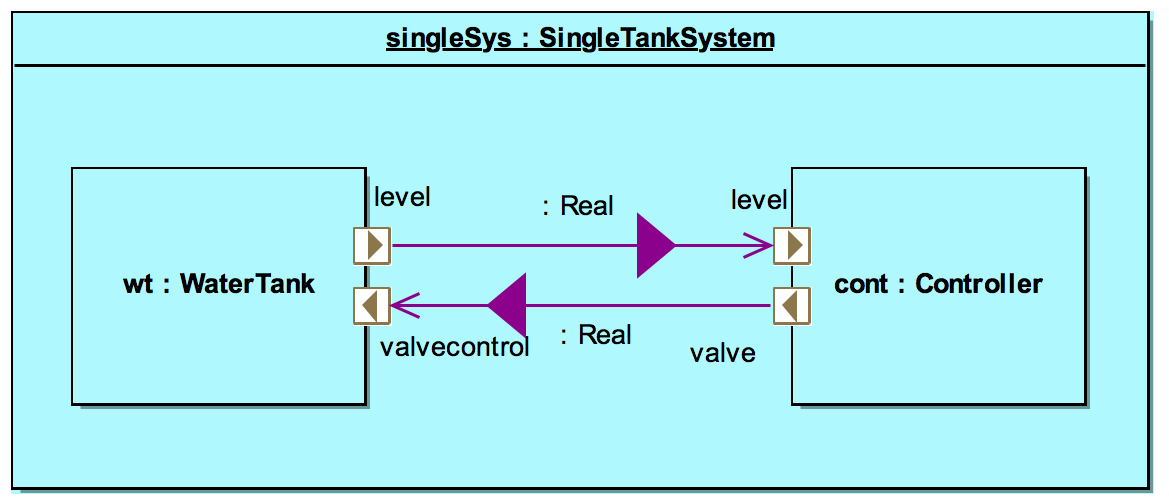
\includegraphics[width=0.75\textwidth]{singletank/sysml_cd.png}
\caption{Connections Diagram defining the Single-tank Water Tank system connections}
\label{fig:singletankcd}
\end{center}
\end{figure}

\subsection{Multi-model}
\label{sec:singletank_into_mm}

\subsubsection{Models}
\label{sec:singletank_into_models}

The SysML model above dictates there are two models: a 20-sim model for the water tank and a VDM-RT model for the controller. This section gives an overview of those models.

\begin{description}
\item[Watertank.emx] The 20-sim model of the \emph{Water Tank} component, shown in Figure~\ref{fig:singletank20-sim}, comprises several sub-components. A flow source is connected to a tank, which fills up at a constant rate. The tank reports the current water level on the \emph{level} port. A valve, controlled by the \emph{valvecontrol} port empties water from the tank into a drain.

\begin{figure}[htbp]
\begin{center}
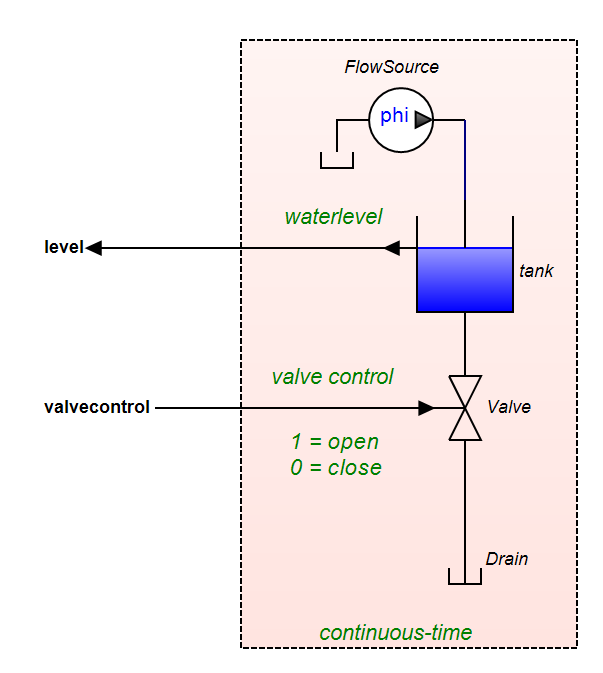
\includegraphics[width=0.5\textwidth]{singletank/20-sim.png}
\caption{20-sim Water Tank component}
\label{fig:singletank20-sim}
\end{center}
\end{figure}

\item[WaterTank.mo] \emph{WaterTank.mo} contains a \emph{SingleWaterTank} model, which has the same external interface as the above \emph{SingleWatertank.emx} model -- as both comply to the FMI \emph{modeldescription.xml} exported format. The model is defined mainly through equations, and so is not shown in this document.
%
%\begin{figure}[htbp]
%\begin{center}
%To Appear %\includegraphics[width=0.5\textwidth]{singletank/om.png}
%\caption{OpenModelica Water Tank component}
%\label{fig:singletankom}
%\end{center}
%\end{figure}

\item[SingleWT] The VDM-RT \emph{SingleWT} controller is a simple model, with an architecture shown in Figure~\ref{fig:singletank20-vdm}. The \emph{System} class owns a \emph{HardwareInterface} instance with RealPorts to receive the sensed water level and send valve control commands. The values are passed to \emph{LevelSensor} and \emph{ValveActuator} objects used by the \emph{Controller} class. The control algorithm compares the level to the \emph{minlevel} and \emph{maxlevel} design parameters and sets the valve control appropriately.
 
\begin{figure}[htbp]
\begin{center}
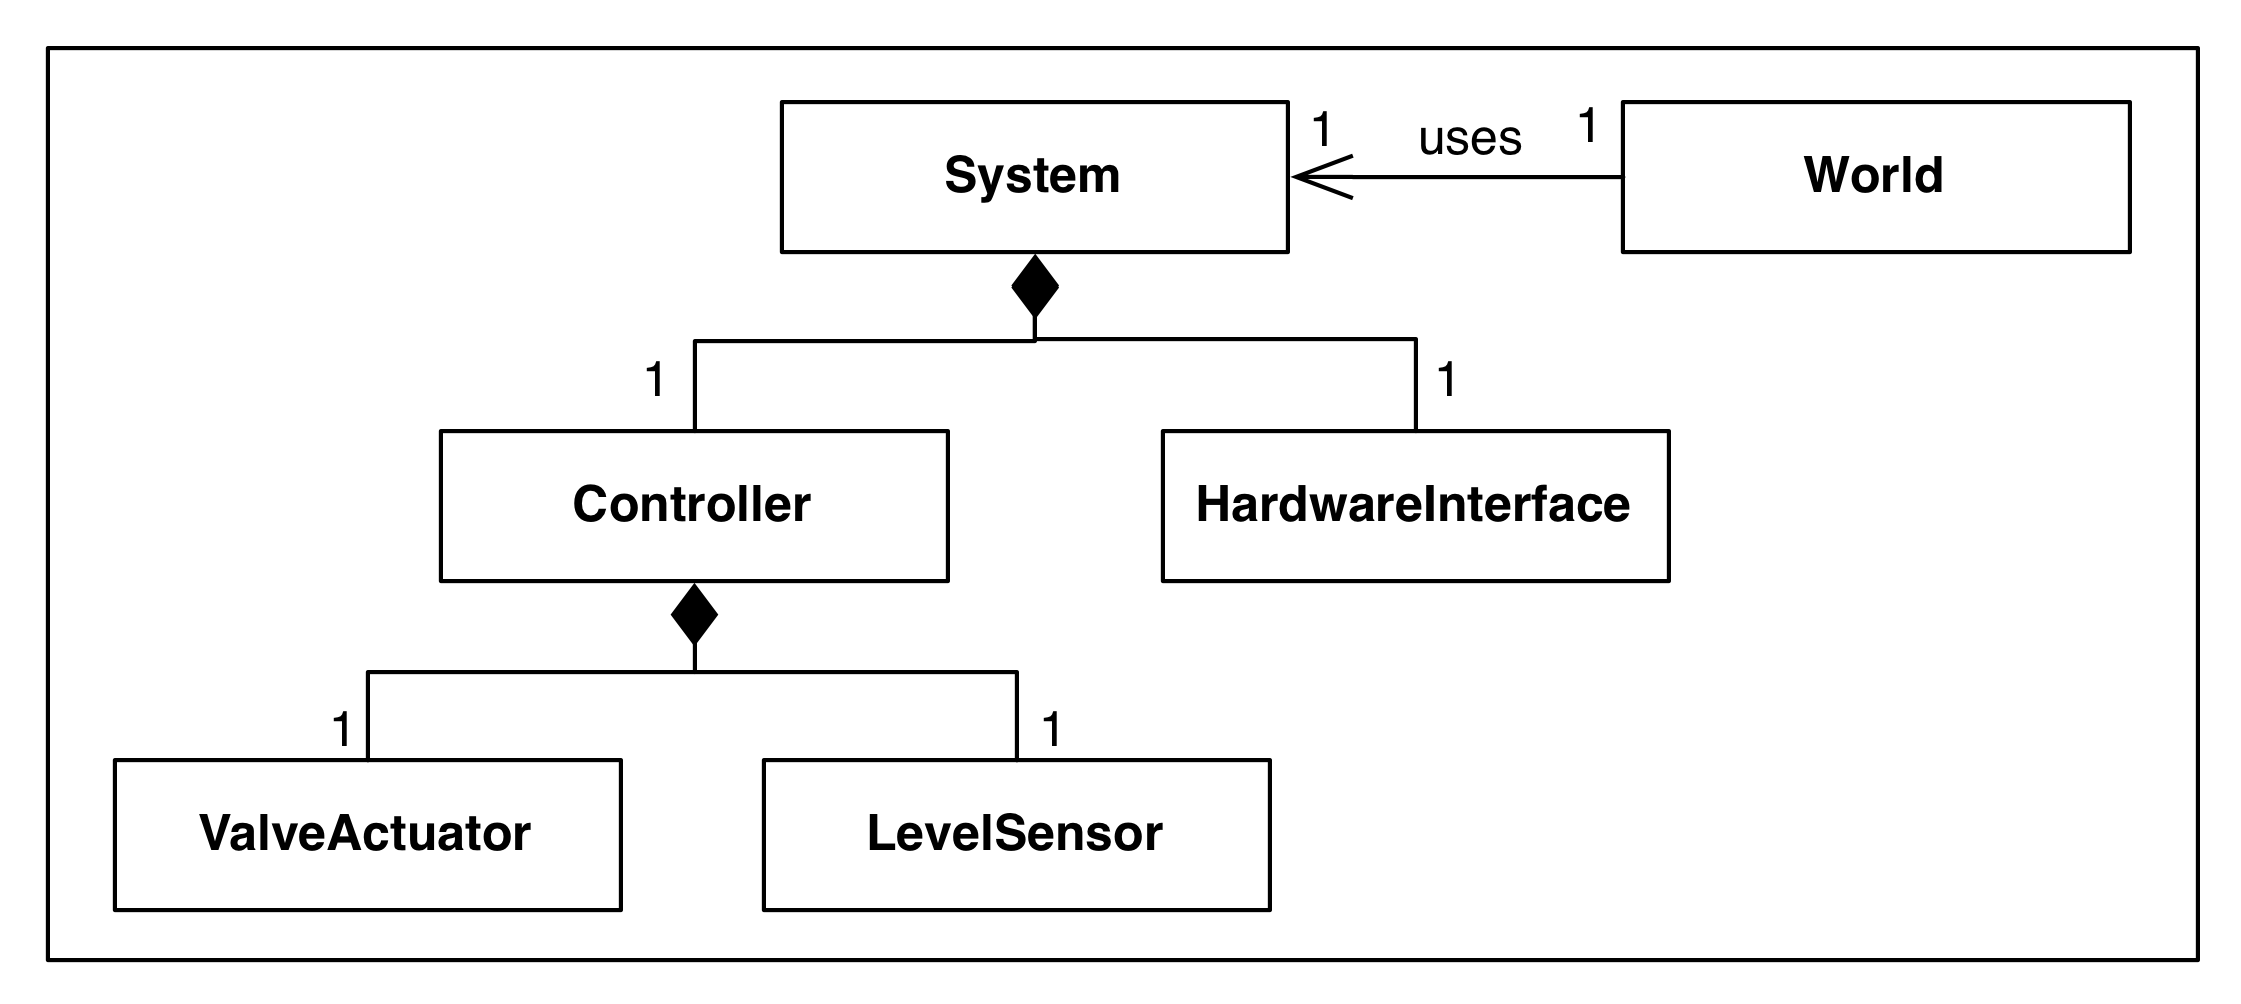
\includegraphics[width=0.755\textwidth]{singletank/vdmrtarch.png}
\caption{VDM-RT model architecture}
\label{fig:singletank20-vdm}
\end{center}
\end{figure}

\end{description}

\subsubsection{Configuration}
\label{sec:singletank_into_conf}
Two multi-models are defined:
\begin{description}
\item[mm] The multi-model \texttt{mm} corresponds to the CD in Section~\ref{sec:singletank_into_sys}. Two connections are defined:

\begin{itemize}
  \item from the \emph{WaterTank} \texttt{level} port to the \emph{Controller} \texttt{level} port; and 
  \item from the \emph{Controller} \texttt{valve} port to the \emph{WaterTank} \texttt{valvecontrol} port. 
\end{itemize}

The FMUs used are \emph{singlewatertank-20sim.fmu} and \emph{SingleWT.fmu}

There are two design parameters in the multi-model -- \texttt{minlevel} and \texttt{maxlevel}, which are defined to be 1.0 and 2.0 respectively. 

\item [mm-OM] An alternative multi-model is defined using the OpenModelica FMU. The connections are identical to the multi-model above, although rather than using the 20-sim FMU, \emph{WaterTank\_SingleWaterTank.fmu} is used.

\end{description}

\subsection{Co-simulation}
\label{sec:singletank_into_co}

A co-simulation experiment is defined for the multi-model -- with a runtime of 30 seconds and using the fixed step size of 0.1 seconds. Simulating using this experiment produces the livestream output shown in Figure~\ref{fig:cosim-graph}.

\begin{figure}[htbp]
\begin{center}
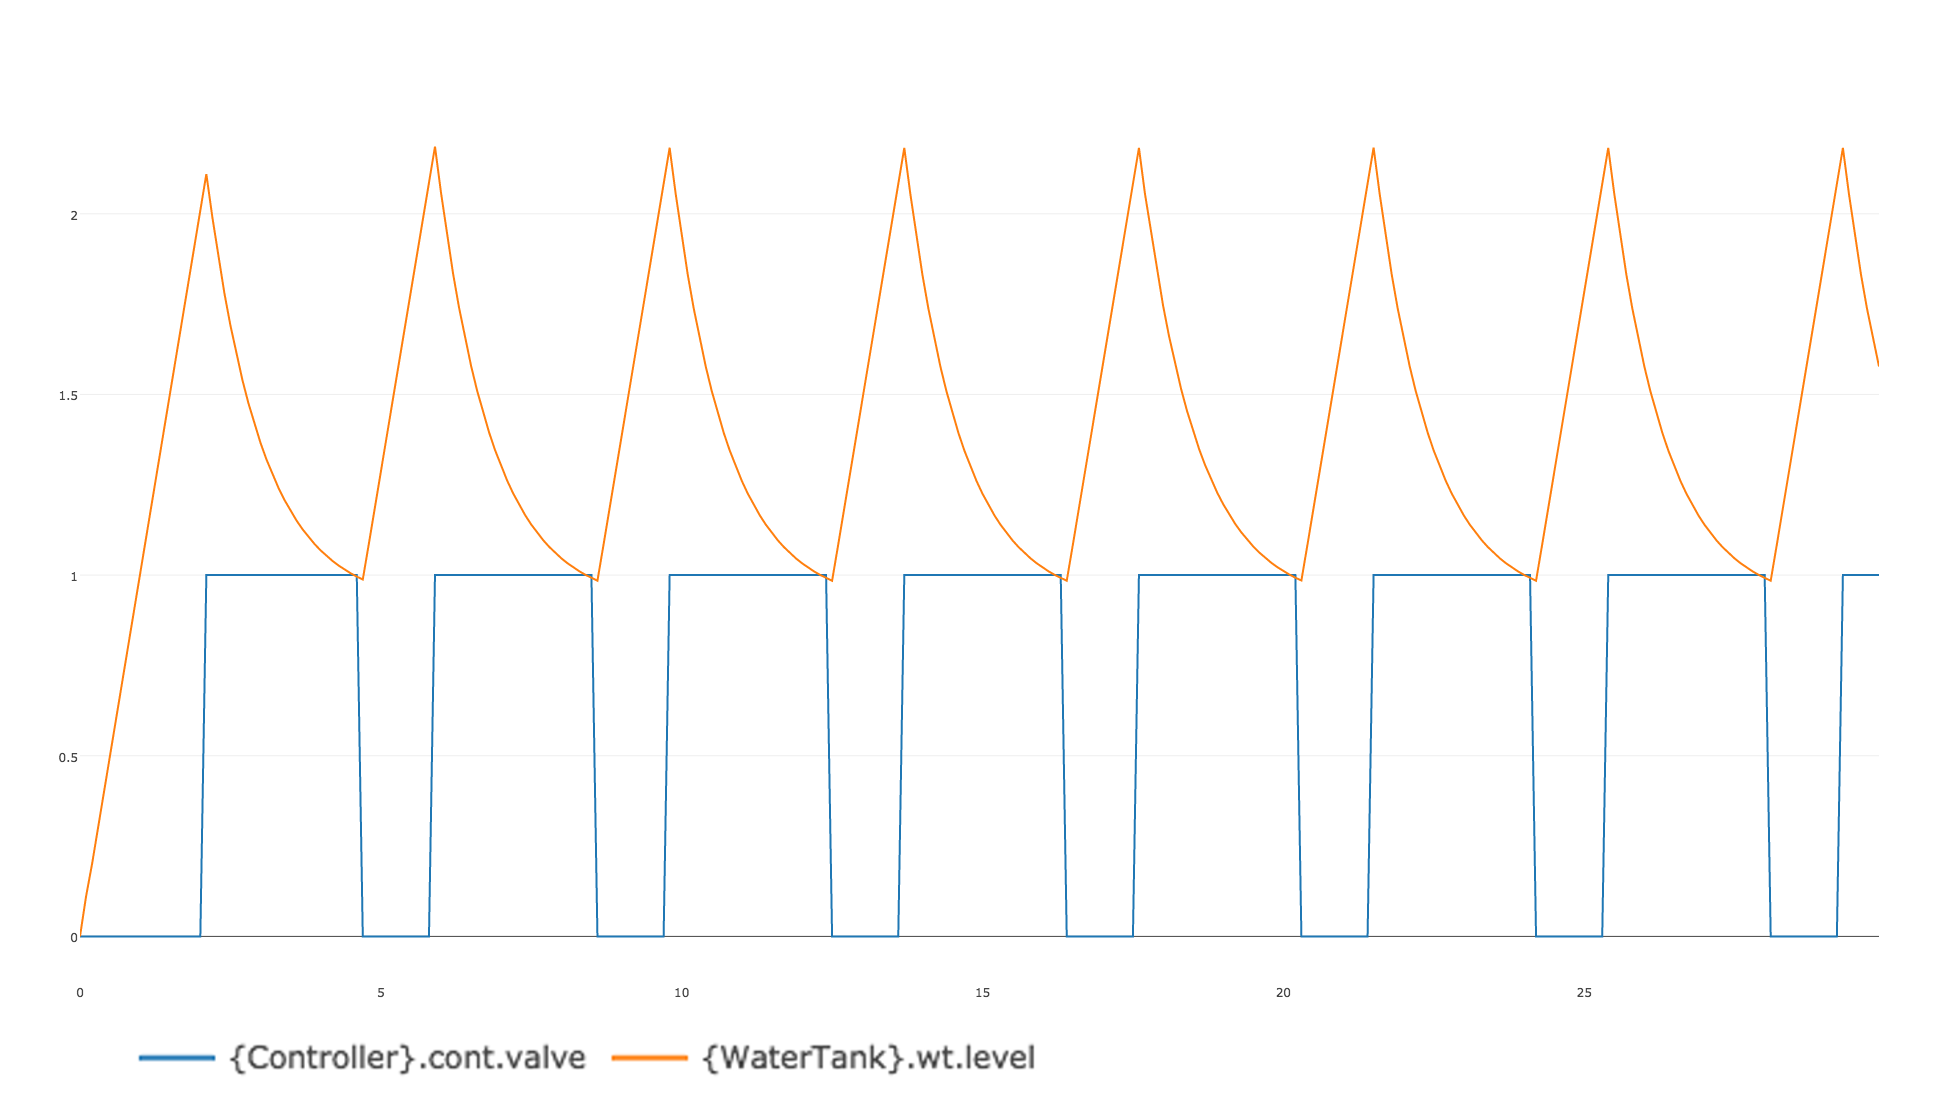
\includegraphics[width=1\textwidth]{singletank/cosim-results.png}
\caption{Co-simulation results for Single-tank Water Tank system}
\label{fig:cosim-graph}
\end{center}
\end{figure}

The graph shows the water level (orange line) and valve control (blue line) values. The water level rises steadily until it reaches 2.0 (the maximum level), at this point the valve control is set to 1.0 and the water level drops to 1.0 (the minimum level). At the minimum level, the valve is closed and the water rises once again. This behaviour repeats through to the end of the simulation. 

\subsection{Analyses and Experiments}

\subsubsection{Design Space Exploration}
\label{sec:singletank_dse}

This pilot supports DSE. We reuse the DSE experiment used in the Three-tank Water Tank Pilot study -- and is briefly described here. For discussion on results obtained, see the Three Tank study in Section~\ref{sec:threetank_dse}.

The experiment varies the two design parameters of the study -- \texttt{minlevel} and \texttt{maxlevel}. These parameter values may be set between $0.2$ and $2.0$ in intervals of $0.2$. A constraint on the parameters (\texttt{{Controller}.cont.maxlevel $>$ {Controller}.cont.minlevel}) ensures that the maximum water value is always larger than the minimum water level. 

Two objectives are defined: \textit{cumulativeDeviation} and \textit{vCount}. The first objective, \textit{cumulativeDeviation}, is to minimise the cumulative deviation from a desired level - set to $1.0$. The second objective, \textit{vCount}, is to minimise the number of valve operations -- i.e. have a lower number of valve state changes. The analysis uses the Pareto method for ranking.

\subsubsection{Code Generation}

The VDM-RT model, \textbf{SingleWT} can be exported from Overture as a C code FMU, in addition to the tool wrapper FMU as used above. The \emph{watertankController-SourceCode.FMU} included in this pilot is obtained directly from Overture using the ``Export Source Code FMU'' option. However, this FMU does not contain binaries for co-simulation and so one may use the \emph{FMU Builder} included in the INTO-CPS Application to compile FMUs for Windows, Mac and Linux. 

This process has been performed and the resultant FMU is included in the pilot in the FMUs folder; \emph{watertankController-Standalone.FMU}. One example experiment available is to switch this FMU for the tool wrapper version -- \emph{SingleWT.FMU} -- and compare results. 